\documentclass[fleqn]{article}

%opening
\title{Reinforcement Learning and the Tic-Tac-Toe Example}
\author{Felix Gutmann, Thomas Vicente, Zsuzsa Holler and Denitsa Panova}
\date{}

\usepackage{graphicx}
\usepackage{listings}
\usepackage{graphicx}
\usepackage{subfigure}
\usepackage[english]{babel}
\usepackage[utf8]{inputenc}
\usepackage{amsmath}
\usepackage{amsfonts}
\usepackage{amssymb}
\usepackage{graphicx}
\usepackage{fancyhdr}
\usepackage{tabularx}
\usepackage{geometry}
\usepackage{setspace}
\usepackage[right]{eurosym}
\usepackage[printonlyused]{acronym}
\usepackage{floatflt}
\usepackage[usenames,dvipsnames]{color}
\usepackage{colortbl}
\usepackage{paralist}
\usepackage{array}
\usepackage{titlesec}
\usepackage{parskip}
\usepackage[right]{eurosym}
    \usepackage[bottom]{footmisc}
%\usepackage{picins}
\usepackage[subfigure,titles]{tocloft}
\usepackage[pdfpagelabels=true]{hyperref}
\lstset{basicstyle=\footnotesize, captionpos=t, breaklines=true, showstringspaces=false, tabsize=2, frame=lines, numbers=left, numberstyle=\tiny, xleftmargin=2em, framexleftmargin=2em}
\usepackage{titlesec}


\begin{document}
\maketitle
\textit{“If we choose to call the Chess-Player a pure machine we must be prepared to 
admit that it is, beyond all comparison, the most wonderful of the inventions of mankind.”}
- \textbf{Edgar Allan Poe}

\section{Introduction}

We have strived to create artificial intelligence (AI) long before we actually had the computing power to do so. Since then, we managed to break almost all such computing boundaries. We have witnessed a lot of algorithms which question which ideas are in the realm of science fiction and which are actually achievable in the near future. The latest accomplishment is the Google AI which beats one of the top GO players in the world, a task long considered impossible. 

In this paper we concentrate on one of the main technique used to create AIs, reinforcement learning (RL) and more specifically Q-learning method. This variation is using exactly the principles of Dynamic Programing (DP). We will focus on its applications for board games. These examples are interesting as they represent a measure for the ability to implement abstract thinking. Although for humans it is natural to learn to master games, the architecture of machines makes them unable to learn with the same flexibility, until recently. There are many computational methods which have been created in order to “teach” the AI how to play successfully. 


In this paper, we will present the theory behind reinforcement learning and its variations. We then present its pratical application to build a tic-tac-toe robot player. After this, we explore, in the context of this implementation, different parametrizations and the resulting strategies. We finally provide a review of other similar applications of reinforcement learning.

\section{Reinforcement Learning}

Aim of machine learning is to create intelligent entities, called agents. Reinforcement Learning is the sub-field specialized in this area. To make a parallel with supervised learning (SL), we can say the agent in SL is taught how to react in a given situation from experience. In RL, there is room for randomness in the choice of the next step. When the action is completed, the agent is told if it has been a good or bad decision by providing negaive or positive reward. The agent learns how to act in the future based on that constant feedback. 

Put in other words, the agent is learning from interacting with its environment and observing what is the outcome of this interaction. However, in most of the cases the agent is not told if his action is good or bad immediately after it has been made. The reward migth come after several additional steps. This leads to the so-called “temporal credit assignment problem”: how to decide which step contributes the most to the success of a game, as the agent does series of decisions before getting the reward. We deal this problem using RL and especially temporal difference learning. We will elaborate more on the topic later on.

\subsection{Reasoning}
The reasoning for RL is simple. Imagine playing the game. Adults analyze the current situation and use their experience to deduce which the next best step is. Young children use experience to a much lower extent. They mostly use the trial-error basis. This is exactly what RL does. When children play they record the success of a specific action. They repeat the better actions more often. However, they might fail to consider their oponent's move. By playing a lot, the kid or the agent learns to consider this and gets a better "cause and effect" idea of the game. 

Consider the following RL algorithm:  

\begin{enumerate}
	\item Agent observes the state (each state is a point)  
	\item An action is undertaken by a decision policy (a function which defines agent's action in a given state) 
	\item The agent receives a scalar reward - a function of state and action (the agent maximizes total reward over a long horizon)  
	\item  Information about the reward in the particular state is recorded 
\end{enumerate}

If the game is long enough, the agent will have enough information to perform well in the environment.    

\subsection{Exploitation vs Exploration}
A crucial trade-off in RL is to choose between exploitation and exploration. If the agent has performed a specific action in the past and has received a positive reward, then most likely he will prefer to choose it later on: this is the exploitation of the acquired knowledge. However, this prevents the algorithm from finding new paths which could possibly be better. Thus we need to explore new paths to some extent. The most common way to achieve a good balance between these two aspects is to partially randomize in order not to get stuck in a local optima.

\subsection{Value Function}
The value functions are the key to solve the “temporal credit assignment problem” which we have discussed previously. They depend on the state-action pair and estimate how good a particular action is in a given state, or what the return for that action is expected to be. The value functions indicate the long-run premium in contrast to the reward which is the immediate gain of an action. The following notations are used: $s$ for state, $\pi$ for policy, $V_\pi(s)$ for  \textbf{value} $s$ and $\pi$, and $Q_\pi(s,a)$ for  \textbf{expected reward} if we undertake action $a$ and if we are at state $s$ and have policy $\pi$.  

Now we need to know how to estimate those value functions in order to understand which is the best reward and consequently which is the best action to take.  

\subsection{Temporal Difference Learning}
Temporal Difference learning (TD) is one of the possible ways to estimate the best actions to take. It is a combination of Monte Carlo ideas and DP ideas. Its Monte Carlo aspect is that the algorithm learns by sampling the environment according to a policy, and the DP side is corresponding to approximating the current estimate by previously learned estimates. There are two types of TD based on when the reward is estimated: at the end of the game or at each state. 

 \begin{tabbing}
 	\text{} \hspace{5.5cm} \= \= \= \text{}   \\
 	\\
 	\textbf{Estimating at each state:} 	\>	\>  \>   $V(s_t) = V(s_t) + \alpha [r_{t+1} +\gamma V(s_t+1) -V(s_t)]$ \\
 	\\
\textbf{Estimating at the final stage:} 	\>	\>  \> $V(s_t) = V(s_t) + \alpha [V(s_{t+1}) - V(s_t)]$    \\ 
 \end{tabbing}

where $s_t$ is the current stage;   
$s_t+1$ is the next stage;   
$\alpha$ is the learning rate, a number between 0 and 1 which shows the extent to which the newly acquired information will override the old information;  
$\gamma$ is the discount rate, giving the importance of future rewards, representing idea that future rewards worth less than the current ones;  
$r_{t+1}$ is the observed reward at time t+1

Since the game we have chosen is tic-tac-toe, where one receives a reward only at the end of the game, we concentrate on the latter.  

\subsubsection{On- vs Off-Policy}
The On-Policy is used to learn the \textbf{value of a particular policy}. The update is done by values of the same policy. The policies are usually “soft”, meaning that they ensure exploration of the game's possibilities. This is done by making the algorithm chooses random action (not a greedy-reward-optimizing one) with probability epsilon. 
The Off-Policy learns different policies in order to  \textbf{evaluate behavior and value estimation.} Again the policies should be “soft” in order to promote exploration. Note that in the On-Policy method the update of the estimated value is done strictly based on  \textbf{experience}, whereas in the Off-Policy approach, hypothetical actions are also used. This means that an agent trained by an off-policy method may end up learning strategies that it has not necessarily seen during the learning phase.

\subsection{Q-learning}
Q-learning is a type of Off-Policy TD method. It is a model-free approach to find the $Q$ value function. It can be proven that given sufficiently “soft” policies, it converges with probability 1 to an action-state value function for an arbitrary policy when the following criteria are met: each action is executed in each state an infinite number of times, $\alpha$ is decreased with an appropriate schedule and action-values are stored perfectly.

Moreover, if this approach is used, it is guaranteed that the optimal policy is reached even when actions are selected according to a very exploratory policy.   

The algorithm works in the following manner:  

\begin{enumerate}
	\item Observe the current state, $s$.  
	\item  Choose an action, $a$, for the particular state based on one of the policies
	\item Take the action, and observe the reward, $r$, as well as the new state, $s'$.
	\item  Update the Q-value for the state using the observed reward and the maximum reward possible for the next state.
\end{enumerate}


Updates are done in the following way:  
$$Q(s,a) =  Q(s,a) + \alpha(r + \gamma \max_{\alpha}[Q(s',a')-Q(s,a)])$$   
where $\alpha$ is the learning rate, $\gamma$ is the discount factor and $max_{\alpha}$ is the maximum reward in the following state.   
5. Set the state to the new state, and repeat the process until a terminal state is reached.  
For the tic-tac-toe game, we do not have a reward for every action. Therefore, the value functions coincide. 

\subsection{Q-learning as a DP Algorithm}
We know that the $Q$ value function of each action in a particular state can be expressed as a sum of the rewards of an action in the particular state plus the expected future of the rewards if we continue using the same policy. Moreover, we present the reward function as a value depending on the current state, the current action, and the next state. 
$$Q(s,a) = E[ r_t(s_t, a_t)$$
$$+ \gamma r_{t+1}(s_{t+1}, \arg \max_{a_{t+1}} Q(s_{t+1}, a_{t+1}), s_{t+2})$$
$$+ \gamma^2r_{t+2}(s_{t+2}, \arg \max_{a_{t+2}} Q(s_{t+1}, a_{t+2}), s_{t+3}) + \dots ]$$
If we want to maximize this equation, we can transform the problem, we will look for argmax $Q$, $Q*$ (Watkins, 1989; Watkins and Dayan, 1992). This approach finds $Q*$ iteratively through a forward dynamic model.   
$Q*(s,a) = r + \gamma max_{\alpha}[Q(s,a)]$, which is done in $\alpha$ proportion. Therefore, convergence is guaranteed with probability 1.

\section{Tic-Tac-Toe Game in the RL Framework}

The game:
\begin{itemize}
	\item  2 players (X and O player)
	\item 3-by-3 board
	\item players take turns alternately placing their marks
	\item goal: have three mark in a row, a column or a diagonal
\end{itemize}

We approach the game by using reinforcement learning method with value function (temporal difference learning method):

\begin{itemize}
	\item  the state \textbf{s}: a given position of marks in the table
	\item the value function $\boldsymbol{V(s)}$: for each possible state of the game is taken the estimated probability of winning (We initialized at 0.5)
	\item The $\boldsymbol{Q}$ value function - make greedy moves, in each state make a move which results in the highest value state in the next step
	\item exploration: with some probability (parameter $\epsilon$) make exploratory moves
\end{itemize}

\section{Functioning of the code}
This section describes the code contained in the Appendix. The code is largely based on the implementation of the Innohead team \footnote{sites.google.com/a/innohead.com/wiki/Home/Python/reinforcement-learning---tic-tac-toe0}. Though, we adjusted some parameters and added others to augment the depth of our experimental analysis. ALso we enhanced the GUI (graphical user interface).

The general structure of the code is organized around classes. They are Python structures containing both functions and objects that can belong to the class' environement or to the global environment. Classes allow for functions and variables which are closely related to each other to be stores in one place and thus interact more easily. 

The class  \textbf{State} is creating the actual board with the visual representaion of the values ( \_ , X, and O) and their corresponding tuple keys recognized by the learner algorithm (No Play, Player 1, Player 2). The object takes as input the current actions of the players and fills the table accordingly. It also contains two additional functions. One of them returns whether one of the players won the game and the other one the game checks if the board is full. 

The class  \textbf{Learner} is the most important in the code. It contains the function which enumerates all available actions for a player at a given state. Another function in this class evaluates the gain of a particular state. In particular, the reward of a win is 1, of a loss is -1, and of a tie is 0. The function next\_action is pivot as it determines what will be the next move of the AI. The next move corresponds to the action which, according to the past experience, has the highest value, a function of the value. The value is computed by another part of the code. More precisely, the value of a state is updating using the value of the next state after evaluating the result of the last action. We have also enriched the original code by adding a parameter allowing more or less for randomness in the 'next action' decision process. Whe end-up with the standard Q-learning iteration:
$$\text{value(lastState)} = (1-\alpha)\text{intermediateValue(lastState)} + \alpha \ \text{value(newState)}$$

The class  \textbf{Game} is in charge of the display of the information to the human player. This is also where we choose to let the AI to train against itself and we can specify for how many games as well. Owning to this class we can also record where the players choose to play in the board.

The class  \textbf{Selfplay} creates the oponent player and make two AIs play against each other. The aim is to prepare the AI to play (well) against a human player. We also use this class to evaluate how an AI is performing and how its sequences of actions are converging to the optimal strategy with different sets of parameters. We discuss that in the next section.

While playing the game, the human user is allowed to train the AI with N games with the function g.selfplay(N), where N is a natural number. To play the game call the function g(i,j) which enable you to position your mark on the tic-tac-toe board - i is the row and j is the column.

\section{Parameters and learning behaviour}

In the following we describe the learning behaviour of the two player classes according to changes in parameters. 
In order to study the behaviour of the algorithm we let two robot players play against each other. We observe the wining and draw rates for an increasing number of training games and for both players we record over time how the value of a few of the possible starting states evolve over time. We chose to examine the value of the starting positions for two reasons. First, these positions are reached frequently when playing the game again and again, since in the beginning of the game there are only a limited number of scenarios possible. Consequently, the values of these states are updated frequently and more likely to depict the learning behavior and success of the two players. Second, the evolution of these values well illustrates that while the agents make greedy moves - taking into account only the immediate consequence of actions - the algorithm still achieves strategies which are overall “optimal”. 

First we examine the specification when both player have the same learning parameter. We exclude random choices and let both players decide optimally in a greedy way.\\


\textbf{Figure 1:} Developement of game outcome shares as a function of number of training games
\begin{center}
	\begin{tabular}{cc}
		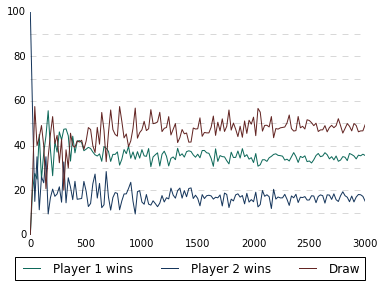
\includegraphics[width=70mm]{alpha02.png} &   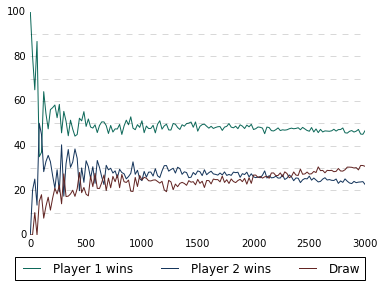
\includegraphics[width=70mm]{alpha08.png} \\
		(a) Outcomes ($\alpha=0.2$, $\epsilon=0$)   & (b) Outcomes ($\alpha=0.8$, $\epsilon=0$)   \\[4pt]
	\end{tabular}
\end{center}

\textbf{Figure 3:} Value function for starting states ($\alpha=0.2$, $\epsilon = 0$)
\begin{center}
	\begin{tabular}{cc}
		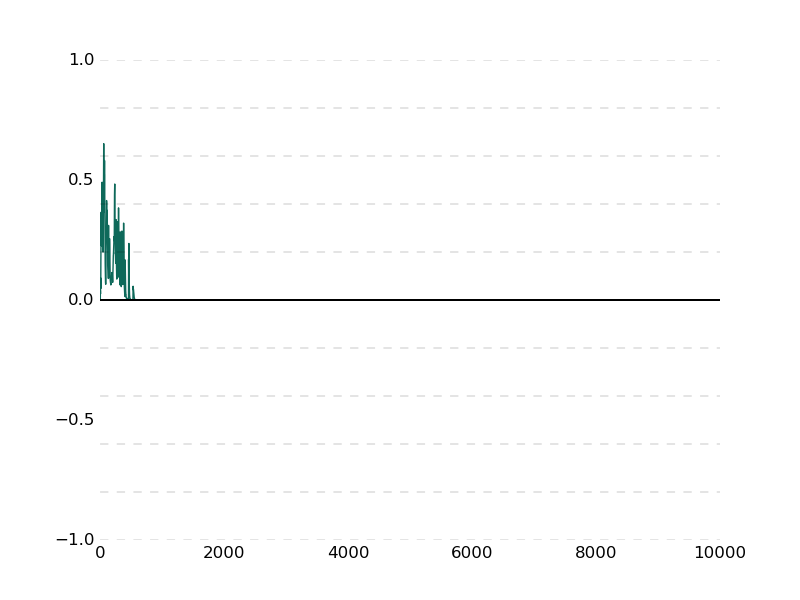
\includegraphics[width=70mm]{player1_0200.png} &   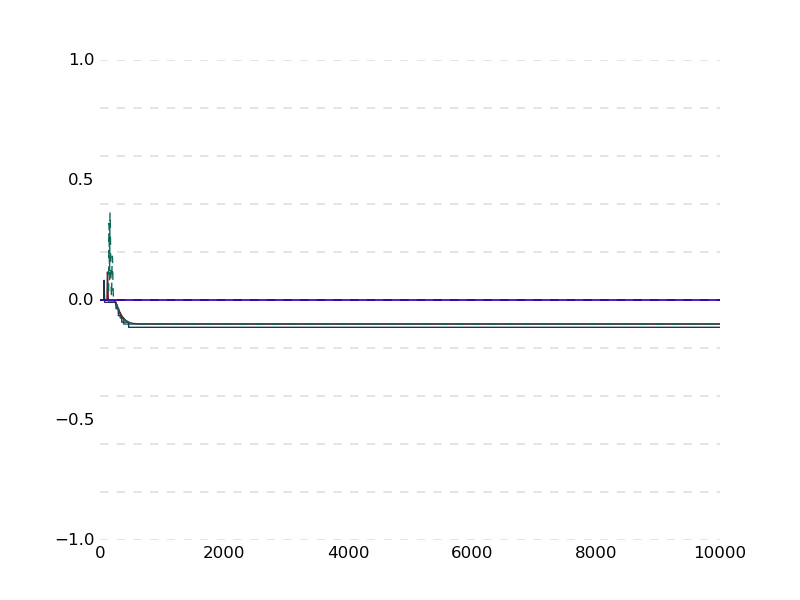
\includegraphics[width=70mm]{player2_0200.png} \\
		(a) Player 1   & (b) Player 2    \\[4pt]
	\end{tabular}
\end{center}

Figure 1 (a) and (b) depict the outcome of games as a function of the number of training games. In general we can observe that the number of shares of draws is increasing for an increasing number of games. For lower learning rates the share of draw games is increasing faster. Furthermore, the development for higher levels of alpha is less volatile. 
It can be seen that the value of most of the states does not change at all for both players. With no randomization both players stuck in a given strategy (a local optimum) which leads to the outcome that the first player wins most of the times while the second player does not find the strategy to beat the first player. In all cases the winning share of game opening player is constantly higher, which makes sense since he has a slight advantage. 

Now we observe what happens with different learning rates if the players make exploratory moves. We set the level of randomisation to 0.02 ( $\epsilon = 0.02$ ). We tried different levels of randomisation and this seems to be a reasonable level for the learning behaviour. The final results of the games looks quite similar as in the no radomisation case, but it can be seen that with randomisation both players explore more strategies so the values of the starting positions are constantly updated.  

\textbf{Figure 2:} Developement of game outcome shares as a function of number of training games
\begin{center}
	\begin{tabular}{cc}
		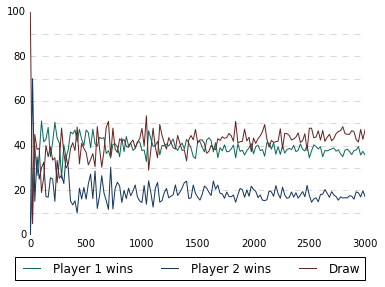
\includegraphics[width=70mm]{alp02eps002.png} &   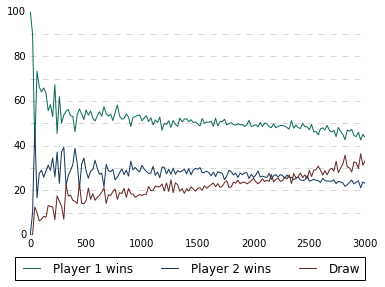
\includegraphics[width=70mm]{alp08eps002.png} \\
		(a) Outcomes ($\alpha=0.2$, $\epsilon=0.02$)   & (b) Outcomes ($\alpha=0.8$, $\epsilon=0.02$)   \\[4pt]
	\end{tabular}
\end{center}

\textbf{Figure 4:} Value function for starting states ($\alpha=0.2$, $\epsilon = 0.02$)
\begin{center}
	\begin{tabular}{cc}
		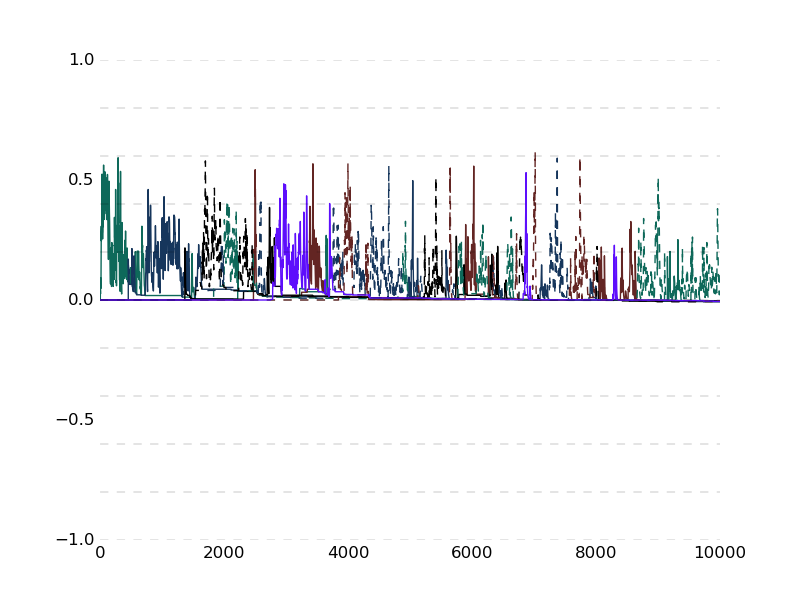
\includegraphics[width=70mm]{player1_0202.png} &   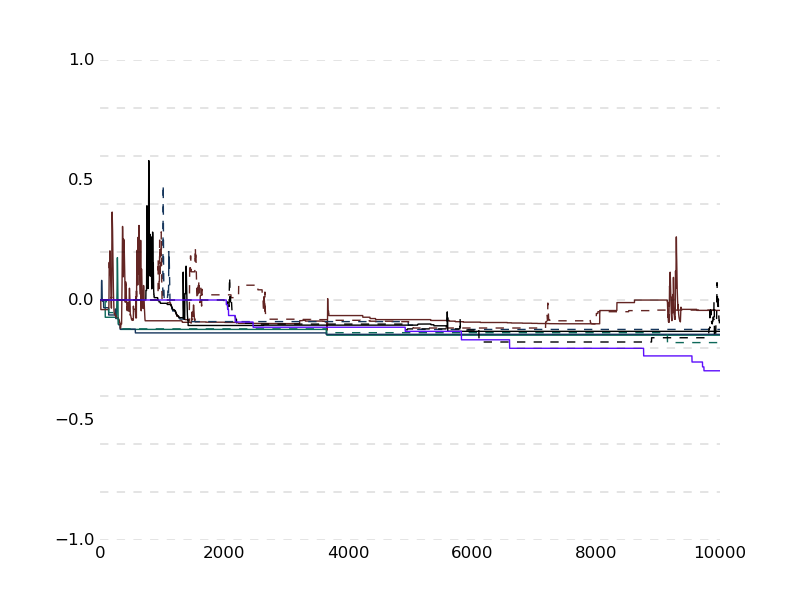
\includegraphics[width=70mm]{player2_0202.png} \\
		(a) Player 1  & (b) Player 2    \\[4pt]
	\end{tabular}
\end{center}

\textbf{Figure 5:} Value function for starting states ($\alpha=0.8$, $\epsilon = 0.02$)
\begin{center}
	\begin{tabular}{cc}
		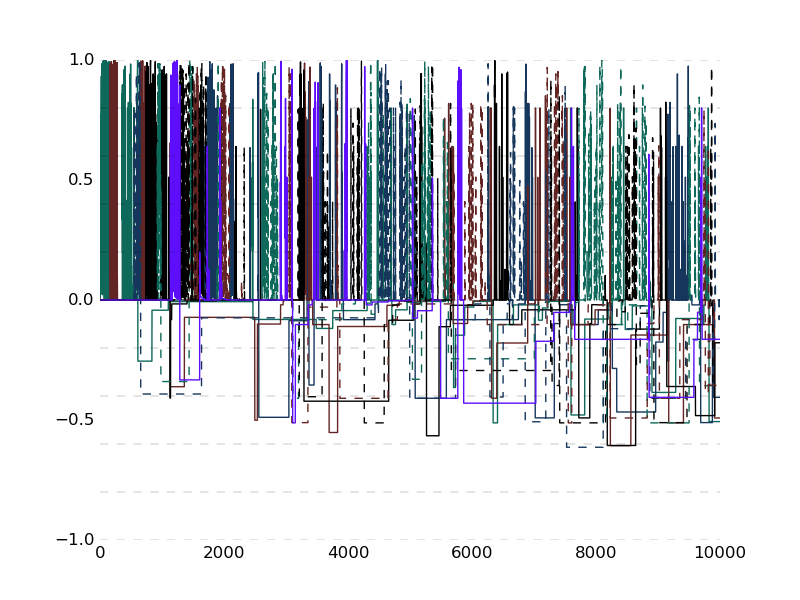
\includegraphics[width=70mm]{player1_0802.png} &   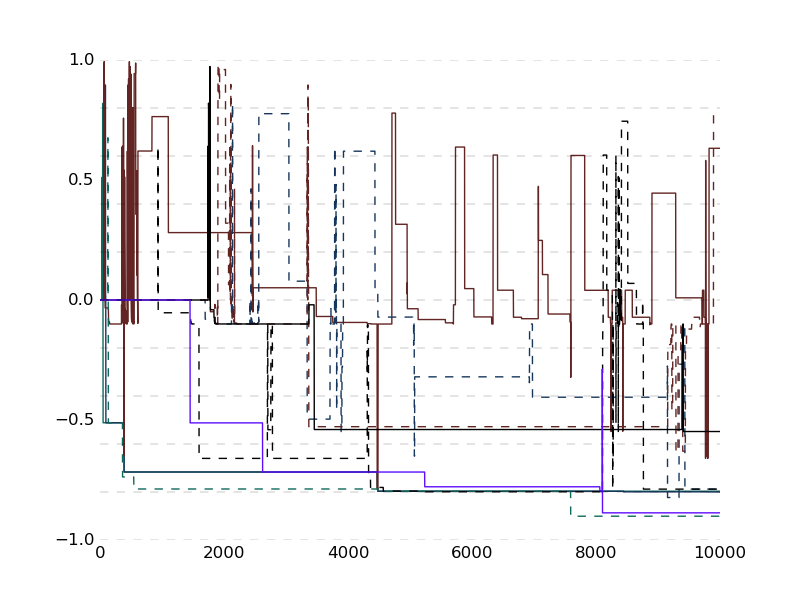
\includegraphics[width=70mm]{player2_0802.png} \\
		(a) Player 1  & (b)  Player 2  \\[4pt]
	\end{tabular}
\end{center}

The first player still performs better in general, but different first moves are distinguished  based on their success rate in case of both players. For the first player, starting in the middle (green dashed line) seems to be slightly better than any other starting point. For the second player,  states which are available after the first player started at the middle are in general disadvantageous. This is not surprising since this is the winning strategy of the first player according to our results. On the other hand, the second player also learned for example that if the first player starts at the corner it is better to put in the middle (brown solid line) than to put next to the first player (green solid line).  Note that the robot trained with no randomization might performed similarly against the other robot player but it did not have this extra information.  If the robot has to play against a human, who does not necessarily play the optimal strategy, this plus information might be very useful. 

With higher learning rate the values are much more volatile, and it seems that the winning rates do not stabilize in 3000 iterations. This is most likely due to the fact that when a player takes a random step a drastic increase or decrease in the value of the state might occur purely by chance. Therefore, too sensitive value estimates are observed and consequently, overall, a slower convergence.

\section{Q-learning applications review}

\subsection{Classical Q-learning}
In this section, we present similar variations of the Q-learning algorithm for other applications.

\subsubsection{Pacman}
The Pacman AI describes a state using a vector of features. The vector actually capture multiple different states simultaneously. The vector entries are real numbers, often 0/1, which are calculated by functions that capture important properties of the state: distance to closest ghost, distance to closest dot, number of ghosts, $1/(distance to dot)^2$, is Pacman in a tunnel? (0/1 example). This information is used to find which actions usually result in good outcomes, and which result in bad. So if in the current state there is a food pellet above the AI, and the AI moves up to eat the food pellet, it will remember that, in this state, moving up and eating the food pellet was a good decision because its score increased. As in the tic-tac-toe exanple, the game is played repeatedly to build a table of memories so the robot gets better. 

\subsubsection{Financial trading}
It is possible to automatically evaluate the best course of n actions among buying, selling, and staying out (do not do anything). This again is done using algorithm's experience and without any prior knowledge of the environment in advance. The Q-learning algorithm is achieved by optimizing different value functions: internal profit, sharp  ratio,  derivative  sharp  ratio. The selection of the right value functions is important to achieve a stable learning algorithm, especially if the environement is unstable. Also, we add auxilary parameter in order to learn the value function - the variance of the environment's variables. It is reported by Du et al. (2009) that this approach leads to better performance in the algorithm  even than the performance achieved using stationary and fixed value functions. 

\subsubsection{Intelligent anti-tank mines}
Mine-carying robots have been designed with sensors determining enemy tanks' direction and velocity (the state). Based on this, two perceptual triggers (actions) are initialized: CAN\_INTERCEPT and NEAR. If CAN\_INTERCEPT is TRUE, then the robot chooses the action INTERCEPT. If NEAR is TRUE, it chooses the action TERMINATE. Otherwise it chooses WAIT. The robot is rewarded if a tank is destroyed after a termination action. The perceptual triggers are reevaluated accordingly to the history of rewards. 

\subsection{Q-learning with approximations}
Q-learning might loose viability with applications having too large state sizes or action spaces. To solve this problem, some applications use function approximations speeding up the learning by providing finite state spaces. There is even possible to work in infinite state spaces.

\subsubsection{Backgammon}
Artificial neural networks are an example of function approximation. They are implemented in Tesauro's backgammon player using TD learning. It is useful for non-deterministic game with smooth and continuous state space where similar board positions have similar values. In contrast, in deterministic games, such as chess, a small difference in board position can have large consequences for the state value. 

\subsubsection{Deepmind}
A recent application by Google DeepMind merged Q-learning with deep learning. Titled "deep reinforcement learning" or "deep Q-networks", it was able to beat humans on Atari games. An astonishing fact is that the agent, actually receiving only the pixel information and the game score as inputs, was able to surpass the performance of all previous algorithms. Actually it achieves a level comparable to that of a professional human tester across a set of 49 games, using the same algorithm, network architecture and hyperparameters. 

The Q-network algorithm combines both the successes of the Q-learning policy research and the Deep Learning ability to map high-dimentional inputs to simpler spaces. In particular, for each game play, the network has as many loss functions as there are potential actions to reach the objective state. Also, to avoid getting stuck in loops and/or local minima, the loss functions are evaluated as the averaged value of different (and not always optimal in a greedy perspective) tries.

\pagebreak
\section*{References}
http://cs229.stanford.edu/proj2009/LvDuZhai.pdf

http://www.cc.gatech.edu/ai/robot-lab/online-publications/iros02-ebeowulf-saho-arkin.pdf

http://www.readcube.com/articles/10.1038%2Fnature14236

Richard Sutton and Andrew Barto (1998). Reinforcement Learning. MIT Press. ISBN 0-585-02445-6

Peng Ding and Tao Mao, Reinforcement Learning in Tic-Tac-Toe Game and Its Similar Variations, Thayer School of Engineering at Dartmouth College  

Sutton, Richard S. and Barto, Andrew G., Reinforcement Learning: An Introduction, MIT Press, 1998  

The Reinforcement Learning Repository, University of Massachusetts, Amherst  

Tesauro, Gerald, Temporal Difference Learning and TD-Gammon, Communications of the Association for Computing Machinery, March 1995 / Vol 38, No. 3  

Imran Ghory, Reinforcement learning in board games, 2004   

Chris Gaskett, Q-learning for Robot Control, 2002

\pagebreak
\section*{Appendix}
	

	
\end{document}